\documentclass[journal,12pt,twocolumn]{IEEEtran}
%

\usepackage{setspace}
\usepackage{gensymb}
\singlespacing

\usepackage{amsmath}
\usepackage{amsthm}
\usepackage{txfonts}
\usepackage{cite}
\usepackage{enumitem}
\usepackage{mathtools}
\usepackage{listings}
    \usepackage{color}                                            %%
    \usepackage{array}                                            %%
    \usepackage{longtable}                                        %%
    \usepackage{calc}                                             %%
    \usepackage{multirow}                                         %%
    \usepackage{hhline}                                           %%
    \usepackage{ifthen}                                           %%
  %optionally (for landscape tables embedded in another document): %%
    \usepackage{lscape}     
\usepackage{multicol}
\usepackage{chngcntr}
\renewcommand\thesection{\arabic{section}}
\renewcommand\thesubsection{\thesection.\arabic{subsection}}
\renewcommand\thesubsubsection{\thesubsection.\arabic{subsubsection}}

\renewcommand\thesectiondis{\arabic{section}}
\renewcommand\thesubsectiondis{\thesectiondis.\arabic{subsection}}
\renewcommand\thesubsubsectiondis{\thesubsectiondis.\arabic{subsubsection}}

% correct bad hyphenation here
\hyphenation{op-tical net-works semi-conduc-tor}
\def\inputGnumericTable{}                                 %%

\lstset{
%language=C,
frame=single, 
breaklines=true,
columns=fullflexible
}

\begin{document}
%


\newtheorem{theorem}{Theorem}[section]
\newtheorem{problem}{Problem}
\newtheorem{proposition}{Proposition}[section]
\newtheorem{lemma}{Lemma}[section]
\newtheorem{corollary}[theorem]{Corollary}
\newtheorem{example}{Example}[section]
\newtheorem{definition}[problem]{Definition}
\newcommand{\BEQA}{\begin{eqnarray}}
\newcommand{\EEQA}{\end{eqnarray}}
\newcommand{\define}{\stackrel{\triangle}{=}}
\bibliographystyle{IEEEtran}
\providecommand{\mbf}{\mathbf}
\providecommand{\pr}[1]{\ensuremath{\Pr\left(#1\right)}}
\providecommand{\qfunc}[1]{\ensuremath{Q\left(#1\right)}}
\providecommand{\sbrak}[1]{\ensuremath{{}\left[#1\right]}}
\providecommand{\lsbrak}[1]{\ensuremath{{}\left[#1\right.}}
\providecommand{\rsbrak}[1]{\ensuremath{{}\left.#1\right]}}
\providecommand{\brak}[1]{\ensuremath{\left(#1\right)}}
\providecommand{\lbrak}[1]{\ensuremath{\left(#1\right.}}
\providecommand{\rbrak}[1]{\ensuremath{\left.#1\right)}}
\providecommand{\cbrak}[1]{\ensuremath{\left\{#1\right\}}}
\providecommand{\lcbrak}[1]{\ensuremath{\left\{#1\right.}}
\providecommand{\rcbrak}[1]{\ensuremath{\left.#1\right\}}}
\theoremstyle{remark}
\newtheorem{rem}{Remark}
\newcommand{\sgn}{\mathop{\mathrm{sgn}}}
\providecommand{\abs}[1]{\left\vert#1\right\vert}
\providecommand{\res}[1]{\Res\displaylimits_{#1}} 
\providecommand{\norm}[1]{\left\lVert#1\right\rVert}
\providecommand{\mtx}[1]{\mathbf{#1}}
\providecommand{\mean}[1]{E\left[ #1 \right]}
\providecommand{\fourier}{\overset{\mathcal{F}}{ \rightleftharpoons}}
\providecommand{\system}{\overset{\mathcal{H}}{ \longleftrightarrow}}
\newcommand{\solution}{\noindent \textbf{Solution: }}
\newcommand{\cosec}{\,\text{cosec}\,}
\providecommand{\dec}[2]{\ensuremath{\overset{#1}{\underset{#2}{\gtrless}}}}
\newcommand{\myvec}[1]{\ensuremath{\begin{pmatrix}#1\end{pmatrix}}}
\newcommand{\cmyvec}[1]{\ensuremath{\begin{pmatrix*}[c]#1\end{pmatrix*}}}
\newcommand{\mydet}[1]{\ensuremath{\begin{vmatrix}#1\end{vmatrix}}}
\newcommand{\proj}[2]{\textbf{proj}_{\vec{#1}}\vec{#2}}
\let\StandardTheFigure\thefigure
\let\vec\mathbf
\title{Assignment - 1 New}
\author{Arjun Jayachandran
\\ MD/2020/702}
% make the title area
\maketitle
\newpage
%\tableofcontents
\bigskip
\renewcommand{\thefigure}{\theenumi}
\renewcommand{\thetable}{\theenumi}
%\renewcommand{\theequation}{\theenumi}
\begin{abstract}
This is a simple document to learn about vectors
\end{abstract}
%Download all python codes 
%
%\begin{lstlisting}
%svn co https://github.com/JayatiD93/trunk/My_solution_design/codes
%\end{lstlisting}
Download all and latex-tikz codes from 
%
\begin{lstlisting}
svn co https://github.com/gadepall/school/trunk/ncert/geometry/figs
\end{lstlisting}
%
\section{Vectors}
\renewcommand{\theequation}{\theenumi}
\begin{enumerate}[label=\thesection.\arabic*.,ref=\thesection.\theenumi]
\numberwithin{equation}{enumi}
\item Draw the graphs of the following equations: 
$$ 3x-4y+6=0 $$
$$ 3x+y-9=0 $$
Also determine the co-ordinates of the vertices of the triangle formed by these lines and the x-axis.
\\
\solution
In Equation 1,
$$ 3x-4y+6=0 $$
$\therefore$
$$ y=\frac{3x+6}{4} $$
Representing this equation graphically. Solutions in Table 1.1.
\begin{table}[h!]
    \centering
    \begin{tabular}{ |c|c|c| } \hline
 x & -2 & 6 \\
 \hline
 $y=\frac{3x+6}{4}$ & 0 & 6 \\ \hline
    \end{tabular}
    \caption{}
    \label{table 1.1}
\end{table}
\\
In Equation 2,
$$ 3x+y+9=0 $$
$\therefore$
$$ y=9-3x $$
Representing this equation graphically. Solutions in Table 1.2.
\begin{table}[h!]
    \centering
    \begin{tabular}{ |c|c|c| } \hline
 x & 0 & 3 \\
 \hline
 $y=9-3x$ & 0 & 6 \\ 
 \hline
    \end{tabular}
    \caption{}
    \label{table 1.2}
\end{table}\\
Plot the points
$$\vec{P}\myvec{6 & 6}$$
$$\vec{Q}\myvec{-2 & 0}$$
$$\vec{R}\myvec{0 & 9}$$
$$\vec{S}\myvec{3 & 0}$$
corresponding
to the solutions in Table 1.1 & 1.2. Draw the lines $\vec{PQ}$ & $\vec{RS} $,
representing
the
equations as shown in Fig. 1.1
\\
In Fig. 1.1, observe that the two lines representing the two equations are
intersecting at the point $$\myvec{2 & 3}$$
Co-ordinates of the vertices of the triangle formed by the lines and the x-axis are 
$$\myvec{2 & 3}$$
$$\myvec{-2 & 0}$$
$$\myvec{3 & 0}$$
\begin{figure}[h]
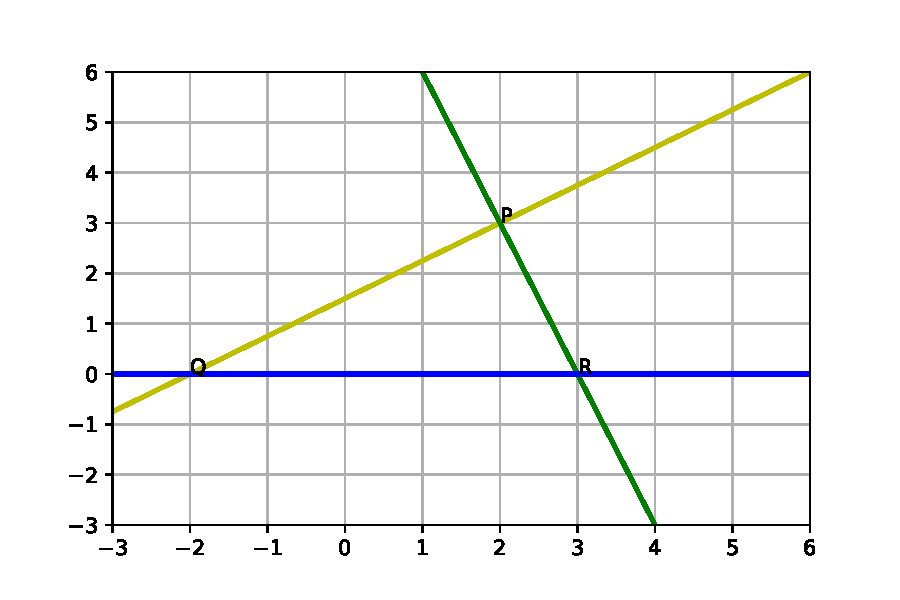
\includegraphics[width=8cm]{line.pdf}
\caption{Two lines representing given equations meet at point $\myvec{2 & 3}$ }.
\end{figure}
\end{enumerate}
\end{document}
